%
% fem.tex
%
% (c) 2020 Prof Dr Andreas Müller, Hochschule Rapperswil
%
\section{Finite Elemente
\label{section:finite-elemente}}
\rhead{Finite Elemente}
Die Technik der finiten Volumina basierte darauf, dass die gesuchte
Funktion durch Integrale über Volumina oder Flächenstücke ersetzt 
werden konnte, zwischen denen lineare Gleichungen gelten.
Dies ist jedoch nicht die einzige denkbare Vorgehensweise.
In diesem Abschnitt zeigen wir, wie gewisse partielle Differentialgleichungen
in ein äquivalentes Minimalprinzip umgewandelt werden können.
Approximiert man die gesuchte Funktion anschliessend durch geeignete
Interpolationspolynome, wird das Minimalproblem zu einem quadratischen
Minimalproblem für die Koeffizienten der Interpolationspolynome,
welches mit Methoden der linearen Algebra gelöst werden kann.

\subsection{Das äquivalente Minimalproblem}
Zur Illustration des Prinzips soll in diesem Abschnitt das Eigenwertproblem
für eine elliptische Differentialgleichung zweiter Ordnung betrachtet werden.

\subsubsection{Ein eindimensionales Problem}
Wir betrachten die Differentialgleichung
\begin{equation}
u''(x) = \lambda u(x)
\label{pde:fem:1dgl}
\end{equation}
auf dem Interval $[a,b]$ mit Randwerten  $u(a)=u(b)=0$
und möchten zeigen, dass eine Lösung gleichzeitig ein stationärer
Punkt des Integrals
\begin{equation}
I(u)
=
\int_a^b u'(x)^2 + \lambda u(x)^2 \,dx
\label{pde:fem:1minimal}
\end{equation}
ist.

\begin{satz}
\label{pde:satz:minimal1}
Eine Funktion $u(x)$ ist genau dann eine Lösung der Differentialgleichung
\eqref{pde:fem:1dgl}, wenn sie das Funktional
$I(u)$ von \eqref{pde:fem:1minimal} minimiert.
\end{satz}

\begin{proof}[Beweis]
Ein Minimum der Funktion $I(u)$ erfüllt die Bedingung, dass jede 
Variation $u(x)+\varepsilon h(x)$ von $u$, die den Randbedingungen genügt,
einen grösseren Wert von $I$ liefert.
Die Ableitung nach $\varepsilon$ verschwindet also an der Stelle
$\varepsilon=0$.
Wir setzen
\[
I(\varepsilon) = I(u(x) + \varepsilon h(x))
\]
mit beliebigen Funktionen $h(x)$, die am Rand verschwinden: $h(a)=h(b)=0$.
\begin{align}
0
=
\frac{dI(\varepsilon)}{d\varepsilon}\bigg|_{\varepsilon=0}
&=
\frac{d}{d\varepsilon}
\int_a^b (u'(x)+\varepsilon h'(x))^2  + (u(x)+\varepsilon h(x))^2\,dx
\bigg|_{\varepsilon=0}
\notag
\\
&=
\int_a^b
2u'(x)h'(x) + 2\varepsilon h'(x)^2
+
2\lambda u(x)h(x) + 2\lambda \varepsilon h(x)^2
\,dx
\bigg|_{\varepsilon=0}
\notag
\\
&=
2
\int_a^b
u'(x)h'(x)
+
\lambda u(x)h(x)
\,dx
\notag
\intertext{Um das Integralprinzip~\ref{pde:XXX} anwenden zu können, darf
nur $h(x)$ vorkommen.
Wir können die Ableitung $h'(x)$ mit Hilfe von partieller Ableitung zum
Verschwinden bringen.}
&=
2\biggl[u'(x)h(x)\biggr]_a^b
-
2\int_a^b u''(x) h(x)\,dx
+
2\int_a^b \lambda u(x) h(x)\,dx.
\notag
\intertext{Der erste Term verschwindet, da $h(x)$ an den Intervallenden
verschwindet:}
&=
2\int_a^b \bigl(-u''(x) +\lambda u(x)\bigr)\,h(x)\,dx.
\label{pde:fem:1integral}
\end{align}
Jetzt kann das Integralprinzip~\ref{pde:XXX} angewendet werden: das
Integral~\eqref{pde:fem:1integral} kann nur dann für alle Funktionen
$h(x)$ verschwinden, wenn
\[
u''(x)=-\lambda u(x)
\]
gilt.
\end{proof}


\subsubsection{Partielle Differentialgleichung auf einem Rechteck}
Das gleiche Prinzip ist auch anwendbar für das Eigenwertproblem
\begin{equation}
\Delta u(x) = \lambda u(x),
\qquad \Delta
=
\frac{\partial^2}{\partial x^2} + \frac{\partial^2}{\partial y^2}
\label{pde:fem:2dgl}
\end{equation}
auf einem Rechteck $\Omega = (a,b)\times (c,d)$, es ist nur nicht
ganz so klar, wie das Problem formuliert werden muss.
Der zentrale Schnitt im Beweis von Satz~\ref{pde:satz:minimal1}
war partielle Integration und die Ausnutzung der Randwerte von $h(x)$.
Indem wir dieses Beispiel auf ein Rechteck verallgemeinern, können
wird die richtige Verallgemeinerung von Satz~\ref{pde:satz:minimal1}
finden.

Da die Funktion von zwei Variablen abhängt, gibt es jetzt nicht nur
eine erste Ableitung sondern deren zwei.
Statt dem Quadrat der ersten Ableitung $u'(x)^2$ werden daher
einen analogen Terme für beide ersten Ableitungen benötigen.
Die Quadratsumme der Ableitungen
\[
(\nabla u)^2
=
\biggl(\frac{\partial u}{\partial x}\biggr)^2
+
\biggl(\frac{\partial u}{\partial y}\biggr)^2
\]
liegt auf der Hand.
In Analogie zum eindimensionalen Problem verwenden wir daher
als Minimalproblem das Funktional
\[
I(u)
=
\int_a^b\int_c^d \nabla u(x)^2 + \lambda u(x)^2\,dy \,dx
\]
und schreiben wieder
\[
I(\varepsilon)
=
I(u + \varepsilon h)
\]
für eine Funktion $h\colon \Omega\to\mathbb R$, die auf dem Rand
verschwindet: also
\[
u(a,y) = u(b,y) = u(x,c) = u(x,d) = 0
\]
für beliebige $x\in[a,b]$ und $y\in[c,d]$.

Die Ableitung nach $\varepsilon$ an der Stelle $\varepsilon=0$ ist
\begin{align*}
\frac{dI(\varepsilon)}{d\varepsilon}\bigg|_{\varepsilon=0}
&=
\frac{d}{d\varepsilon}
\int_a^b\int_c^d
(\nabla u(x)+\varepsilon \nabla h(x))^2
+
\lambda (u(x) + \varepsilon h(x))^2
\,dy \,dx
\bigg|_{\varepsilon=0}
\\
&=
2
\int_a^b\int_c^d
\nabla u(x)\cdot \nabla h(x) +\varepsilon \nabla h(x)^2
+
\lambda u(x) h(x) + \lambda \varepsilon h(x)^2
\,dy \,dx
\bigg|_{\varepsilon=0}
\\
&=
2
\int_a^b\int_c^d
\nabla u(x)\cdot \nabla h(x) + \lambda u(x) h(x)
\,dy \,dx.
\end{align*}

Das erste Term im Integranden enthält wieder Ableitungen der Funktion
$h$, die wir loswerden müssen.

\begin{lemma}
\label{pde:lemma:partint2}
Ist $v(x,y)$ eine beliebige Funktion $v\colon\Omega\to\mathbb R^2$ und
$h\colon\Omega\to\mathbb R$. 
Dann gilt für das Integral von $v\cdot\nabla u$ die partielle
Integrationsformel
\begin{align}
\int_a^b\int_c^d v(x,y)\cdot \nabla h(x,y)\,dy\,dx
&=
\int_c^d
v_x(b,y) h(b,y)
-
v_x(a,y) h(a,y)
\,dy
\notag
\\
&\qquad
+
\int_a^b
v_y(x,d) h(x,d)
-
v_y(x,c) h(x,c)
\,dx
\notag
\\
&\qquad
-\int_a^b\int_c^d
\frac{\partial v_x}{\partial x}+\frac{\partial v_y}{\partial y}
\,dy\,dx
\label{pde:fem:part2d}
\end{align}
\end{lemma}

\begin{proof}[Beweis]
\definecolor{orange}{rgb}{1,0.6,0.2}
\definecolor{gruen}{rgb}{0.2,0.6,0.2}
\definecolor{magenta}{rgb}{0.9,0.2,0.4}
\definecolor{azure}{rgb}{0,0.2,1}
Wir teilen das Integral mit Hilfe von
\[
v(x,y)\cdot\nabla h(x,y) = 
v_x(x,y) \, \frac{\partial h}{\partial x}(x,y)
+
v_y(x,y) \, \frac{\partial h}{\partial x}(x,y)
\]
in zwei Summanden
\[
\int_a^b\int_c^dv\cdot\nabla h \,dy\,dx
=
\int_a^b\int_c^dv_x \frac{\partial h}{\partial x} \,dy\,dx
+
\int_a^b\int_c^dv_y \frac{\partial h}{\partial y} \,dy\,dx
=
I_1+I_2
\]
auf, die wir separat berechnen können.
Für den ersten Summanden erhalten wir
\begin{align}
I_1
&=
\int_a^b\int_c^d v_x(x,y) \frac{\partial h}{\partial x}(x,y)\,dy\,dx
\notag
\\
&=
\int_c^d
\int_a^b
v_x(x,y) \frac{\partial h}{\partial x}(x,y)
\,dx
\,dy
\notag
\\
&=
\int_c^d
\biggl[
v_x(x,y) h(x,y)
\biggr]_a^b
-
\int_a^b \frac{\partial v_x}{\partial x}(x,y) h(x,y)
\,dx
\,dy
\notag
\\
&=
\int_c^d
v_x(b,y) h(b,y)
-
v_x(a,y) h(a,y)
-
\int_a^b \frac{\partial v_x}{\partial x}(x,y) h(x,y)
\,dx
\,dy
\notag
\\
&=
\int_c^d
{\color{magenta}
v_x(b,y) h(b,y)}
{\color{azure}
\mathstrut
-
v_x(a,y) h(a,y)}
\,dy
-
\int_a^b
\int_c^d
\frac{\partial v_x}{\partial x}(x,y) h(x,y)
\,dy
\,dx.
\label{buch:pde:part2dI1}
\intertext{%
Die zweite Summe ist noch einfacher, weil es gar nicht erst notwendig ist,
die Integrationsreihenfolge zu ändern:}
I_2
&=
\int_a^b\int_c^d v_y(x,y)\frac{\partial h}{\partial y}\,dy\,dx
\notag
\\
&=
\int_a^b
\biggl[ v_y(x,y) h(x,y)\biggr]_c^d
-
\int_c^d
\frac{\partial v_y}{\partial y} h(x,y)
\,dy
\,dx
\notag
\\
&=
\int_a^b
{\color{gruen}
v_y(x,d)h(x,d)}
{\color{orange}\mathstrut
-v_y(x,c)h(x,c)}
\,dx
-
\int_a^b
\int_c^d
\frac{\partial v_y}{\partial y} h(x,y)
\,dy
\,dx
\label{buch:pde:part2dI2}
\end{align}
Die beiden Terme zusammen geben genau die im Lemma behauptete Formel.
\end{proof}

\begin{figure}
\centering
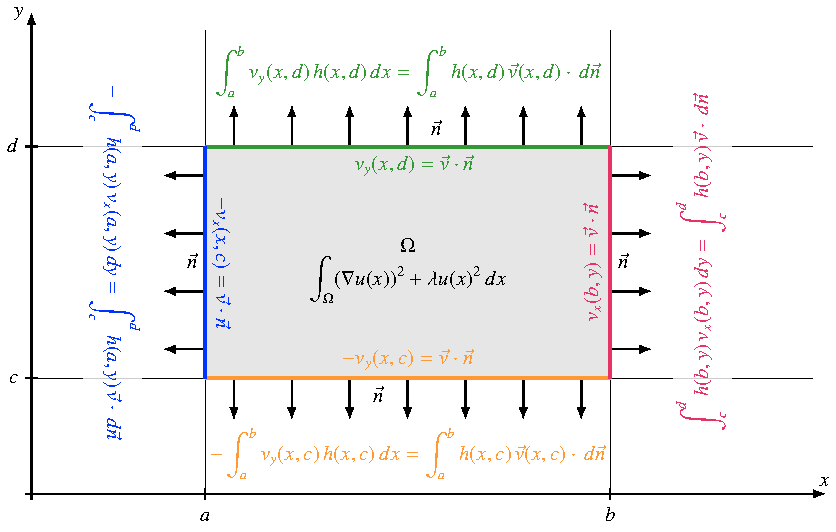
\includegraphics{chapters/70-pde/images/2dpart.pdf}
\caption{Die Randterme des Integrals \eqref{pde:fem:part2d}  können
als ein Flussintegral über den Rand des Rechtecks geschrieben werden.
Dazu müssen die Integrale über die einzelnen Kanten des Rechtecks einzeln
als Flussintegrale über die Kante geschrieben werden.
Die Terme werden auch in den Gleichungen
\eqref{buch:pde:part2dI1} und \eqref{buch:pde:part2dI2}
mit den gleichen Farben hervorgehoben.
\label{buch:pde:pfadintegral}}
\end{figure}
Der erste Integral auf der rechten Seite von Lemma~\ref{pde:lemma:partint2}
kombiniert Integrale von $v_x(x,y) h(x,y)$ über die beiden vertikalen Kanten 
des Rechtecks, während das zweite Integral die Integrale von
$v_y(x,y)h(x,y)$ über die horizontalen Kanten kombiniert (siehe auch
Abbildung~\ref{buch:pde:pfadintegral}.
Schreibt man $\vec{n}(x,y)$ für die nach aussen zeigende Normale auf den Rand 
des Rechtecks, dann können diese Integrale alle einheitlich geschrieben
werden.
\begin{center}
\definecolor{orange}{rgb}{1,0.6,0.2}
\definecolor{gruen}{rgb}{0.2,0.6,0.2}
\definecolor{magenta}{rgb}{0.9,0.2,0.4}
\definecolor{azure}{rgb}{0,0.2,1}
\begin{tabular}{l >{$}c<{$} >{$}l<{$}}
Kante& &\text{Integrand}
\\[2pt]
\hline
\\[-7pt]
\color{orange}untere Kante
	&y=c
	&         - v_x(x,c)h(x,c) = h(x,c) \, \vec{v}(x,c) \cdot \vec{n}(x,c)
\\[4pt]
\color{gruen}obere Kante
	&y=d
	&\phantom{-}v_x(x,d)h(x,d) = h(x,d) \, \vec{v}(x,d) \cdot \vec{n}(x,d)
\\[4pt]
\color{azure}linke Kante
	&x=a
	&         - v_y(a,y)h(a,y) = h(a,y) \, \vec{v}(a,y) \cdot \vec{n}(a,y)
\\[4pt]
\color{magenta}rechte Kante
	&x=b
 	&\phantom{-}v_y(b,y)h(b,y) = h(b,y) \, \vec{v}(b,y) \cdot \vec{n}(b,y)
\\[4pt]
\hline
\end{tabular}
\end{center}
Es folgt also, dass die einfachen Integrale in 
Lemma~\ref{pde:lemma:partint2} das Integral
\[
\int_{\partial\Omega} \vec{v}(x,y) h(x,y) \cdot d\vec{n}
\]
ist.

Nach diesen Vorarbeiten können wir jetzt das zur Differentialgleichung
\eqref{pde:fem:2dgl} gehörige äquivalente Minimalprinzip formulieren.

\begin{satz}
Die Funktion $u\colon\Omega\to\mathbb R$ ist genau dann eine Lösung der
Differentialgleichung
\[
\Delta u =\lambda u
\]
wenn sie das Funktional
\[
I(u)
=
\int_{\Omega} \nabla u(x,y)^2 + \lambda u(x,y)^2 \,dx\,dy
\]
minimiert.
\end{satz}

\begin{proof}[Beweis]
Die Ableitung von $I(\varepsilon)$ an der Stelle $\varepsilon=0$
wurde früher schon berechnet, das Integral~\eqref{pde:fem:part2d}
muss jetzt mit Hilfe der Formel für die partielle Integration
von Lemma~\ref{pde:lemma:partint2} umgeformt werden.
Dazu setzen wir $\vec{v}=\nabla u$ und erhalten für
\[
\frac{\partial v_x}{\partial x}
+
\frac{\partial v_y}{\partial y}
=
\frac{\partial^2 u}{\partial x^2}
+
\frac{\partial^2 u}{\partial y^2}
=
\Delta u.
\]
Es folgt
\begin{align*}
0
&=
\int_{\partial\Omega} \nabla u(x,y) h(x,y) \cdot d\vec{n}
-
\int_{\Omega} \Delta u(x,y) h(x,y)\,dx\,dy
+
\int_{\Omega} \lambda u(x,y) h(x,y)\,dx\,dy
\\
&=
-
\int_{\Omega} \bigl(\Delta u(x,y)-\lambda u(x,y)\bigr) h(x,y)\,dx\,dy.
\end{align*}
Dies gilt genau dann für jede Funktion $h$, wenn
\[
\Delta u = \lambda u,
\]
wenn also $u$ eine Lösung des Eigenwertproblems ist.
\end{proof}

\subsection{Approximation
\label{pde:fem:subsection:approximation}}

\subsection{Quadratische Minimalprobleme}
Die Approximation von Abschnitt~\ref{pde:fem:subsection:approximation}
wandelt das äquivalente Minimalproblem einer partiellen Differentialgleichung
um in ein Minimalproblem für die Koeffizienten der Approximation.
Um die Koeffiziente zu bestimmen, kann man also versuchen, das
Minimalproblem für die endlich vielen Approximationskoeffizienten zu
bestimmen.
Das besondere am Minimalproblem ist, dass es sich um ein quadratisches
Minimalproblem handelt.

\begin{lemma}
\label{pde:fem:gradq}
Sei $A$ eine symmetrische $n\times n$-Matrix, dann ist der Gradient der
Funktion $Q(x) = x^t Ax$
\[
\operatorname{grad}Q(x)
=
\nabla Q(x)
=
2Ax.
\]
\end{lemma}

\begin{proof}[Beweis]
Die Ableitung nach der Variablen $x_i$ ist
\begin{align*}
\frac{\partial}{\partial x_i} Q(x)
&=
\frac{\partial x^t}{\partial x_i} Ax
+
x^t A \frac{\partial x}{\partial x_i}
\\
&=
e_i^t Ax
+
x^tAe_i
=
e_i^t Ax
+
e_i^t Ax
=
2e_i^t Ax
\end{align*}
wegen der Symmetrie der Matrix $A$.
Das Skalarprodukt $e_i^t Ax$ ist die $i$-te Komponente des Vektors $Ax$.
Der Gradient ist der Vektor bestehend aus diesen Komponenten, also
$\operatorname{grad}Q(x) = Ax$.
\end{proof}

\begin{satz}
Seien $A$ und $B$ positiv definite Matrizen.
Dann ist der Vektor $x$ eine Lösung der Gleichung
\[
Ax=\lambda Bx+c
\]
genau dann, wenn er den Ausdruck
\[
I(x)
=
x^tAx - \lambda x^tBx - c^tx
\]
minimiert.
\end{satz}

\begin{proof}[Beweis]
Am Minimum von $I(x)$ verschwindet der Gradient.
Der Gradient der quadratischen Terme ist in Lemma~\ref{pde:fem:gradq}
bereits bestimmt worden.
Der Gradient des linearen Terms ist
\begin{align*}
\frac{\partial}{\partial x_i}c^tx
&=
\frac{\partial}{\partial x_i}\sum_{k=1}^n c_kx_k
=
\sum_{k=1}^n c_k\frac{\partial x_k}{\partial x_i}
=
\sum_{k=1}^n c_k\delta_{ki}
=
c_i
\\
\Rightarrow\qquad
\operatorname{grad}c^tx&=c.
\end{align*}
Damit kann jetzt der Gradient von $I(x)$ bestimmt werden, er ist
\begin{align*}
0=\operatorname{grad}I(x)
&=
2Ax - 2\lambda Bx - c
\\
\Leftrightarrow
\qquad
\qquad
Ax&=\lambda Bx+c.
\end{align*}
Durch Multiplikation mit $B^{-1}$ wird daraus die Gleichung
\[
B^{-1}Ax=\lambda x + B^{-1}c.
\]
\end{proof}




